\documentclass[a4paper]{article}
\usepackage[T1]{fontenc}
\usepackage[utf8]{inputenc}
\usepackage[english,italian]{babel}
\usepackage{graphicx}
\usepackage{amsmath}


\begin{document}
\author{Flavio Sarchione}
\title{Progetto Robotica Aerospaziale: Missione su Venere}
\maketitle
\newpage

\part{Introduzione}
\pagestyle{plain}

L'obiettivo del progetto è quello di elaborare una missione interplanetaria dalla Terra a Venere. Questa è divisa in due fasi: la prima studia la rotta necessaria per raggiungere Venere, mentre la seconda riguarda il ritorno sulla Terra.

Nella prima parte del viaggio, la sonda è situata su un'orbita geostazionaria equatoriale, posta ad una distanza di 200Km dalla superficie. Una volta accesi i motori, essa inizia il viaggio per Venere, con lo scopo di raggiungerla e situarsi in un'orbita stazionaria polare, posta ad una distanza di 500Km dalla superficie del pianeta target.
Inoltre, per il viaggio d'andata, è richiesto che la navicella sfrutti gli effetti della fionda gravitazionale, permettendo un'ottimizzazione in termini di consumi di carburante. Nel progetto, questo fenomeno viene sfruttato una sola volta, aumentando l'energia cinetica della sonda attraverso un passaggio ravvicinato con lo stesso Venere. Conseguenza di ciò, come si vedrà successivamente, è quello di ottenere un'orbita sempre eliocentrica avente un periodo orbitale molto simile a quello di Venere, permettendo così un nuovo incontro ravvicinato, con successiva accensione dei propulsori, in modo da garantire che la navicella resti in orbita attorno il pianeta. A questo punto, dopo un paio di manovre, arrivati nell'orbita desiderata polare, devo garantire che resti su di essa per una durata minima di un mese. Raggiunte queste condizioni, la missione d'andata può ritenersi conclusa.

Nella seconda parte del viaggio, la sonda è chiamata a tornare sulla stessa orbita geostazionaria di partenza.
In questo caso è richiesto che il viaggio di ritorno sia un trasferimento diretto di Hohmann. Una volta giunti sull'orbita finale terrestre, si può ritenere la missione di rientro conclusa.

Di seguito, verrà spiegato come si è svolto il progetto, partendo prima dalla creazione del sistema solare per poi passare allo svolgimento del calcolo della rotta della navicella.
\newpage
\part{Creazione Sistema Solare}
\pagestyle{plain}

\paragraph{Introduzione al problema\newline}
Per la generazione del Sistema Solare, bisogna conoscere la posizione dei pianeti. Per fare ciò, ci dobbiamo riferire a dei dati di riferimento. Infatti, lo standard usato è il J2000. Questo consiste nella posizione esatta dei pianeti nel giorno 1 Gennaio 2000 alle ore 12.
I dati riportati sono parametri orbitali, cioè parametri utili a ricostruire l'orbita e la posizione esatta in essa del pianeta soggetto. 
Questi sono in totale 6: \newline
[\textit{i}] = Inclinazione dell'orbita \newline [$\Omega$] =  Longitudine del nodo ascendente \newline [$\omega$] = Argomento del periasse \newline
[\textit{a}] = Semiasse maggiore \newline [\textit{e}] = Eccentricità orbitale \newline [$\theta$] = Anomalia vera \newline \newline
Ovviamente, tutti questi parametri sono ottenuti partendo da un sistema di riferimento, dove il Sole è l'origine di esso. In più, la stella rappresenta il fuoco di tutte le orbite dei pianeti. Per questo, i parametri orbitali sono ottenuti riferendosi proprio a questo sistema di riferimento, che per semplicità chiameremo ''frame Sole''.
Infatti, di tutti i 6 parametri, il semiasse maggiore e eccentricità generano l'orbita ellittica 2D, mentre i dati di longitudine del nodo ascendente, argomento del periasse e inclinazione dell'orbita ci danno informazione di come l'orbita è orientata in 3D rispetto il frame Sole.
L'ultimo parametro, l'anomalia vera, ci da la posizione nell'orbita del pianeta rispetto al punto di perielio.
\begin{figure}[htbp]
\centering
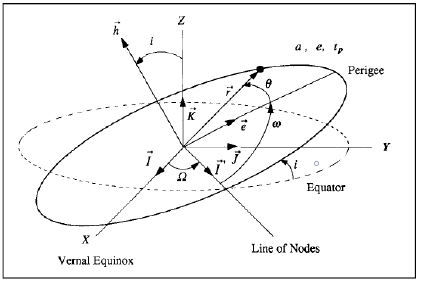
\includegraphics[width=1\textwidth]{Parametri_orbitali.png}
\caption{Rappresentazione grafica dei parametri orbitali.}
\end{figure}

\paragraph{Algoritmo generazione delle orbite\newline}
Per prima cosa, dobbiamo definire matematicamente come si passa dal sistema di riferimento del Sole a quello pianeta. \newline Il sistema di riferimento del Sole coincide col piano dell'ecclittica, dove l'origine di questo è il Sole stesso, mentre i tre assi cartesiani sono ottenuti in modo tale che X e Y siano sul piano dell'ecclittica e Z costruita di conseguenza.
Mentre, per un'orbita generale di ogni pianeta, definiamo un piano di riferimento in cui giace l'orbita stessa, dove il Sole è il fuoco dell'ellisse e centro di un nuovo sistema di riferimento solidale al piano, definito in modo tale che l'asse X sia l'asse che collega il fuoco al perielio, Z sia perpendicolare uscente al piano in accordo con l'asse Y parallelo al vettore velocità del pianeta nel punto di periasse.
Quindi, sfruttando questa definizione, i dati di riferimento J2000 forniscono i tre angoli di rotazione per passare da coordinate \textit{riferimento orbita pianeta} a coordinate \textit{riferimento sole}.

Matematicamente, possiamo esprimere il tutto attraverso questa semplice formula: \newline
\[
\begin{bmatrix}
x \\
y \\
z \\
\end{bmatrix}_{sun} = {[T(\omega)]}^{Z} \cdot {[T(\textit{i})]}^{X} \cdot {[T(\Omega)]}^{Z} \cdot
\begin{bmatrix}
x  \\
y \\
z \\
\end{bmatrix}_{orb}
{;}
\begin{bmatrix}
x \\
y \\
z \\
\end{bmatrix}_{sun} = {[T(\omega,\textit{i},\Omega)]}_{planet}^{sun} \cdot
\begin{bmatrix}
x  \\
y \\
z \\
\end{bmatrix}_{orb}
\]\newline
Dove, la matrice di rotazione finale risulterà essere:\newline
\[
{[T(\omega,\textit{i},\Omega)]}_{orb}^{sun} = 
\begin{bmatrix}
c(\Omega)c(\omega)-s(\Omega)s(\omega)c(\textit{i}) & c(\omega)s(\Omega)+c(\Omega)s(\omega)c(\textit{i}) & s(\omega)s(\textit{i}) \\
-c(\Omega)s(\omega)-s(\Omega)c(\omega)c(\textit{i}) & -s(\Omega)s(\omega)-c(\Omega)c(\omega)c(\textit{i}) & s(\textit{i})c(\omega) \\
s(\Omega)s(\textit{i}) & -s(\textit{i})c(\Omega) & c(\textit{i}) \\
\end{bmatrix}
\]\newline
Dove c(x) = cos(x) e s(x) = sin(x).\newline
Nel codice del progetto, la matrice di trasformazione è stata implementata nella funzione matlab \textit{\textbf{euler\_T.m}}, dov'è effettuato questo calcolo come sopra descritto. Inolte, oltre ad essere richiamato per creare le orbite dei pieneti, è stato sfruttato anche in altre circostanze, quali ad esempio usato nella creazione delle rotte durante il volo ravvicinato e traiettorie di uscita/ingresso iperboliche.
Infine, la gestione e la creazione vera delle traiettorie è lasciata eseguire dalla funzione \textit{\textbf{gener\_orb.m}}. I passi per la creazione sono 2:
\subparagraph{Passo 1\newline}
Per generare l'orbita, si è partiti dalla conoscenza del semiasse maggiore e dall'eccentricità orbitale, per poi calcolare il valore di:
\[
\begin{cases}
p = a \cdot (1-e^2) \\
r(\theta(t)) = \frac{p}{1+e\cdot cos(\theta(t))}
\end{cases}
\]\newline
dove p rappresenta il valore di semiraggio medio, mentre r($\theta$(t)) rappresenta il modulo del vettore distanza del pianeta-origine, in un fissato istante di tempo, rappresentato attraverso il valore di anomalia vera.
\subparagraph{Passo 2\newline}
Dalla conoscenza del modulo del vettore posizione, si è creato in modo iterativo una matrice di dati, dove ogni riga rappresenta le tre coordinate cartesiane riferite rispetto il sistema riferimento Sole. Algoritmicamente, il calcolo eseguito è:
\[
\begin{bmatrix}
x \\
y \\
z \\
\end{bmatrix}_{sun}^{T} = {[T(\omega,\textit{i},\Omega)]}_{orb}^{sun} \cdot r(\theta(t)) \cdot
\begin{bmatrix}
cos(\theta(t)) \\
sin(\theta(t)) \\
0 \\
\end{bmatrix}
\]\newline
Dove il valore di $\theta$(t) si è fatto simulare da 0 a 2$\pi$. Il risultato finale è:
\begin{figure}[htbp]
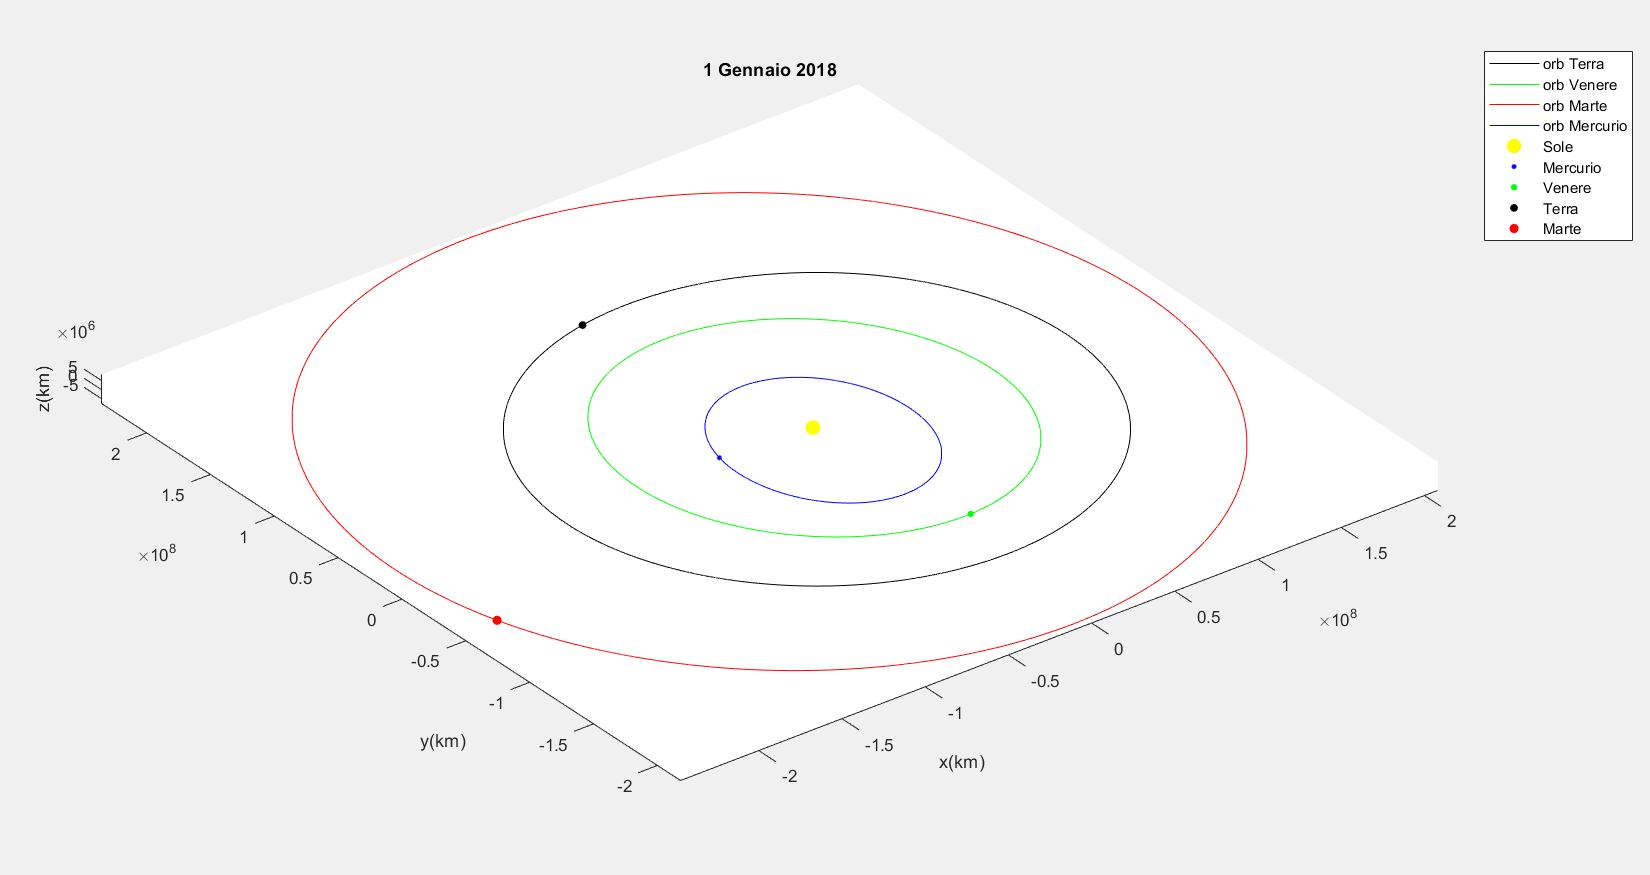
\includegraphics[width=1\textwidth]{Sistema_solareJ2018.png}
\caption{Rappresentazione del Sistema solare il giorno 1 Gennaio 2018}
\end{figure}

\paragraph{Nota generazione parametri orbitali\newline}
Come già detto in precedenza, per costruire le orbite dei pianeti, si devono conoscere i 6 parametri orbitali che determinano la geometria della traiettoria, l'orientazione 3D e la posizione del pianeta stesso. Questi dati sono tutti tabellati in uno standard chiamato J2000 e, per ottenere i dati nel 1 Gennaio 2018 alle ore 12 (che chiameremo per semplicità J2018), si sono fatte alcune ipotesi ed un calcolo semplice: l'ipotesi importante è che le traiettorie compreso il frame di riferimento non varino negli anni, cioè conoscere la struttura orbitale nel 1 Gennaio 2000 ci permette di conoscere esattamente l'orbita anche 18 anni dopo, l'unica differenza risiede nel parametro \textit{anomalia vera $\theta$}, poiché essa consiste nella conoscenza esatta della posizione del pianeta.\newline
Per ottenere questo dato, il calcolo eseguito è semplice:\newline
per prima cosa bisogna passare dalla conoscenza dell'anomalia vera all'anomalia eccentrica:\newline
\[
tan(\frac{E}{2}) = \sqrt{\frac{1-e}{1+e}} \cdot \tan(\frac{f}{2})
\]
per poi calcolare l'anomalia media:
\[
M(t) = E(t) - \textit{e}\cdot sin(E(t))
\]
Questi passaggi sono ''obbligati'', poiché l'anomalia media è descritta da una legge lineare nel tempo (mentre l'anomalia vera non è enunciabile attraverso una legge temporale lineare):
\[
M(t_{2}) = M(t_{1})+n\cdot(t_{2}-t_{1})
\]
dove n è definito moto medio del pianeta, espresso in $\frac{rad}{s}$. \newline Poichè siamo interessati a conoscere la posizione dei pianeti 18 anni dopo, $M(t_{1})$ è il valore nel giorno J2000, $M(t_{2})$ è il valore nel giorno J2018 ed infine $\Delta(t) = t_{2}-t_{1}$ è la distanza temporale calcolata in secondi:
\[
\begin{cases}
\Delta(t) = \textit{annog} \cdot 18 \\
dove \textit{  annog} = 31557600 [s]
\end{cases}
\]
Nota: Ovviamente, una volta calcolata l'anomalia media il 1 Gennaio 2018, si usano le formule inverse per passare al valore di anomalia vera. Algoritmicamente, la funzione usata per la conversione è \textit{\textbf{kepler1.m}}.

\newpage
\part{Prima parte volo: Terra-Venere}
\paragraph{Introduzione\newline}
Il volo di andata consiste in 3 fasi fondamentali: uscita dalla sfera d'influenza terrestre (SOI), volo interplanetario con fly-by su Venere, ingresso sfera d'influenza di Venere e parcheggio su orbita polare.\newline L'ipotesi importante durante il volo è quella di considerare la SOI come un limite dove, all'interno di essa la navicella risente della sola influenza del pianeta, al di fuori dell'influenza del Sole. Con questo criterio, i calcoli eseguiti si basano sullo studio del moto di due corpi. \newline Altra ipotesi importante è quella di considerare la geometria del pianeta come una sfera avente per raggio il raggio medio del corpo celeste.
\paragraph{Analisi del volo\newline}
La missione d'andata deve soddisfare una specifica importante: bisogna fare in modo che la navicella esegua almeno un volo ravvicinato con uno o più pianeti. Nel progetto, viene eseguito un solo fly-by, sfruttando proprio il pianeta target Venere. Quindi, per poter studiare il volo totale c'è bisogno di considerare non solo l'obiettivo finale, ma anche la traiettoria del fly-by. \newline La prima cosa che si deve garantire è che la navicella, una volta uscita dalla SOI terrestre, incontri venere in un punto prefissato. Per far questo, si sfrutta la teoria di Lambert, il quale dati due punti interspaziali desiderati, l'intervallo temporale richiesto e il pianeta di riferimento del moto, restituisce dati utili per costruire l'orbita che passa per quei due punti. \newline La funzione che viene usata \textit{lambert.m} restituisce i vettori velocità e non i parametri orbitali. Per ottenerli, si sfruttano le equazioni di conversione [r,v] -> [$\omega, \Omega, \theta, a, i, e$] descritte in seguito e raccolte nella libreria \textit{rv\_to\_orb.m}. \newline Le equazioni di conversione consistono in:
\[
\begin{cases}
a = -\frac{\mu}{2E} \\
e = \sqrt{1+\frac{2Eh^{2}}{\mu^{2}}} \\
i = cos^{-1}(\frac{\mathbf{\hat{k} \cdot h}}{h}) \\
\Omega = \begin{cases}
cos^{-1}(\mathbf{\hat{i} \cdot \hat{n}}) & \textit{se $\mathbf{\hat{n}\cdot \hat{j}} > 0$}\\
2\pi - cos^{-1}(\mathbf{\hat{i} \cdot \hat{n}})  & \textit{se $\mathbf{\hat{n}\cdot \hat{j}} < 0$} \end{cases} \\
\omega = \begin{cases}
cos^{-1}(\frac{\mathbf{\hat{n} \cdot e}}{e}) & \textit{se $\mathbf{e \cdot \hat{k}} >0$} \\
2\pi - cos^{-1}(\frac{\mathbf{\hat{n} \cdot e}}{e}) & \textit{se $\mathbf{e \cdot \hat{k}} <0$} \end{cases} \\
\theta = \begin{cases}
cos^{-1}(\frac{\mathbf{{e} \cdot r}}{er}) & \textit{se $\mathbf{r \cdot v} >0$} \\
2\pi - cos^{-1}(\frac{\mathbf{{e} \cdot r}}{er}) & \textit{se $\mathbf{r \cdot v} <0$} \end{cases} \\
\textit{dove $\mathbf{\hat{n} = \frac{\hat{k} \times h}{|\hat{k} \times h|}}$} 
\end{cases}
\]
Per le coordinate spaziali, si sono scelti dei punti ai limiti delle SOI, calcolati in previsione anche della parte finale del volo.
\newpage
\subparagraph{Sistema di riferimento pianeta\newline} Per poter svolgere i calcoli bisogna definire, oltre ai sistemi di riferimento Sole e Orbita, anche un sistema di riferimento pianeta, utile per descrivere il moto e le traiettorie della navicella all'interno della SOI. \newline Questo nuovo sistema di riferimento possiede l'asse Z parallelo all'asse Z orbitale, mentre l'asse X è orientato nella stessa direzione del vettore posizione descritto in coordinate orbitali. Con questa scelta, risulta anche che l'asse Y è parallelo al vettore velocità, sempre descritto nel frame orbitale. Quindi, risulta evidente che la matrice di rotazione che ci permette di passare da frame pianeta a frame orbita è una semplice rotazione standard lungo l'asse Z di un angolo pari all'anomalia vera del pianeta. Tuttavia, bisogna anche considerare una differenza non trascurabile: nel processo di trasformazione le origini dei frame \textit{orbita} e \textit{pianeta} non coincidono. Per ovviare a questo problema, si passa ad una scrittura in coordinate omogenee, dove la matrice di trasformazione risulta una $\Re^{4x4}$. Essa contiene non solo informazioni sulla rotazione, ma anche della traslazione, permettendo, così, una velocità maggiore nei calcoli. \newline Scritto il vettore posizione del pianeta in coordinate orbitali $[r_{x}$ $r_{y}$ $r_{z}]^{T}$, matematicamente avrò:
\[
\begin{bmatrix}
x \\
y \\
z \\
1 \\
\end{bmatrix}_{orb} = \begin{bmatrix}
[T(\theta)]^{Z} & \begin{bmatrix}
r_{x} \\
r_{y} \\
r_{z} \\
\end{bmatrix} \\
[\text{0  0  0}] & 1 \\
\end{bmatrix} \begin{bmatrix}
x \\
y \\
z \\
1 \\
\end{bmatrix}_{planet} = [C^{Z}(\theta)]_{planet}^{orb} \cdot \begin{bmatrix}
x \\
y \\
z \\
1 \\
\end{bmatrix}_{planet}
\]
Questa stessa formula viene eseguita per trasformare anche le velocità, a patto di una piccola modifica:
\[
\begin{bmatrix}
v_{x} \\
v_{y} \\
v_{z} \\
0 \\
\end{bmatrix}_{orb} = \begin{bmatrix}
[T(\theta)]^{Z} & \begin{bmatrix}
r_{x} \\
r_{y} \\
r_{z} \\
\end{bmatrix} \\
[\text{0  0  0}] & 1 \\
\end{bmatrix} \begin{bmatrix}
v_{x} \\
v_{y} \\
v_{z} \\
0 \\
\end{bmatrix}_{planet} = [C^{Z}(\theta)]_{planet}^{orb} \cdot \begin{bmatrix}
v_{x} \\
v_{y} \\
v_{z} \\
0 \\
\end{bmatrix}_{planet}
\]
A questo punto, abbiamo tutti gli strumenti matematici per la generazione delle orbite.
\subparagraph{Idea calcolo punti per eq. Lambert\newline}
Come già precedentemente descritto, per calcolare la prima orbita interplanetaria si sfutta l'equazione di Lambert. I vettori passati nella funzione sono coordinate situate sulla superficie delle relative sfere della SOI. Si sfrutta, per il calcolo di questi punti, la scrittura attraverso coordinate polari.\newline Il calcolo è:
\[
p_{earth} = R_{SOI\_earth}\begin{bmatrix}
cos(\theta_{long})cos(\theta_{lat}) \\
cos(\theta_{long})sin(\theta_{lat}) \\
sin(\theta_{long}) \\
\end{bmatrix}_{earth}
\]
\[
p_{venus} = R_{SOI\_venus}\begin{bmatrix}
cos(\theta_{long})cos(\theta_{lat}) \\
cos(\theta_{long})sin(\theta_{lat}) \\
sin(\theta_{long}) \\
\end{bmatrix}_{venus}
\]
dove $R_{SOI\_earth} = 0.929e^{6}km$,  $R_{SOI\_venus} = 0.615e^{6}km$.
\subparagraph{Orbite finali di volo: considerazioni e risultati grafici\newline}
Per calcolare le coordinate di Lambert, ho bisogno di fare alcune ipotesi: la prima cosa che si deve garantire è che tutte le orbite siano ammissibili (cioè devo evitare che la navicella impatti sul pianeta e che le velocità, ottenute dall'eq. di Lambert, siano fisicamente realizzabili), poi devo assicurarmi che avvenga il volo ravvicinato (lo è se i punti sulla superficie della SOI sono tali da far avvenire il fenomeno) e, avvenuto il fly-by, devo garantire un'orbita tale da avere un nuovo incontro con Venere (questa la posso rispettare avendo un periodo orbitale della navicella molto simile a quella di Venere). \newline Garantite queste specifiche, una richiesta ulteriore è sull'orbita iperbolica di cattura di Venere: si desidererebbe una traiettoria iperbolica con il periasse uguale al raggio di Venere sommato 500km, distanza richiesta dall'orbita di parcheggio finale. \newline Sulla base di tutte queste richieste, si sono calcolati i valori di \textit{$p_{earth}$} e \textit{$p_{venus}$} andando a settare e controllare tutti gli angoli a essi associati. \newline Infine, si è anche calcolata la traiettoria d'uscita terrestre.
I risultati grafici sono:
\begin{figure}[htbp]
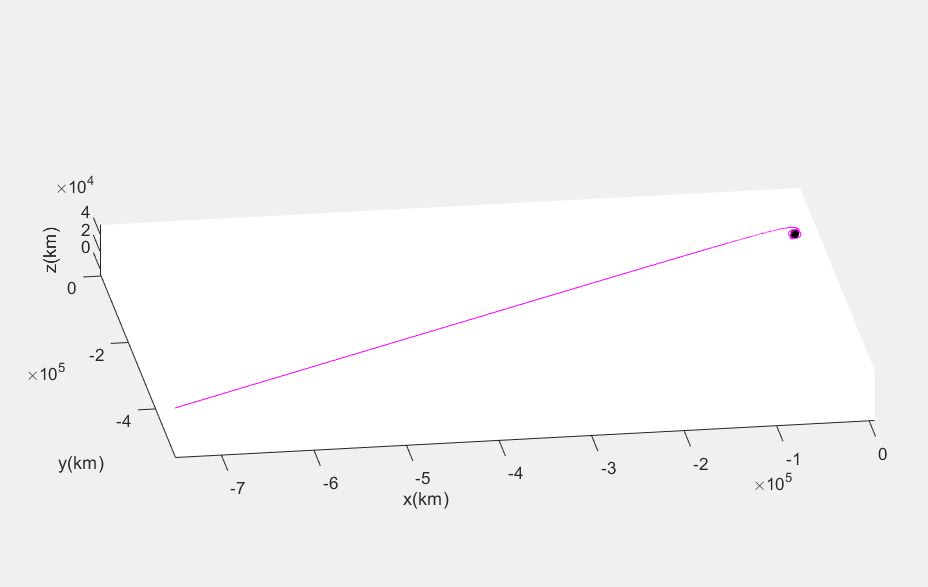
\includegraphics[width=1\textwidth]{Uscita_SOI_terra.png}
\caption{Orbite uscite attrazione terrestre: \newline $R_{cyrcle\_orb}$ = 6578 km, $e_{cyrcle\_orb} = 0$ \newline $a_{hyp\_orb} = -2.2e4$ km, $e_{hyp\_orb}$ = 1.297}
\end{figure}\newline
\begin{figure}[htbp]
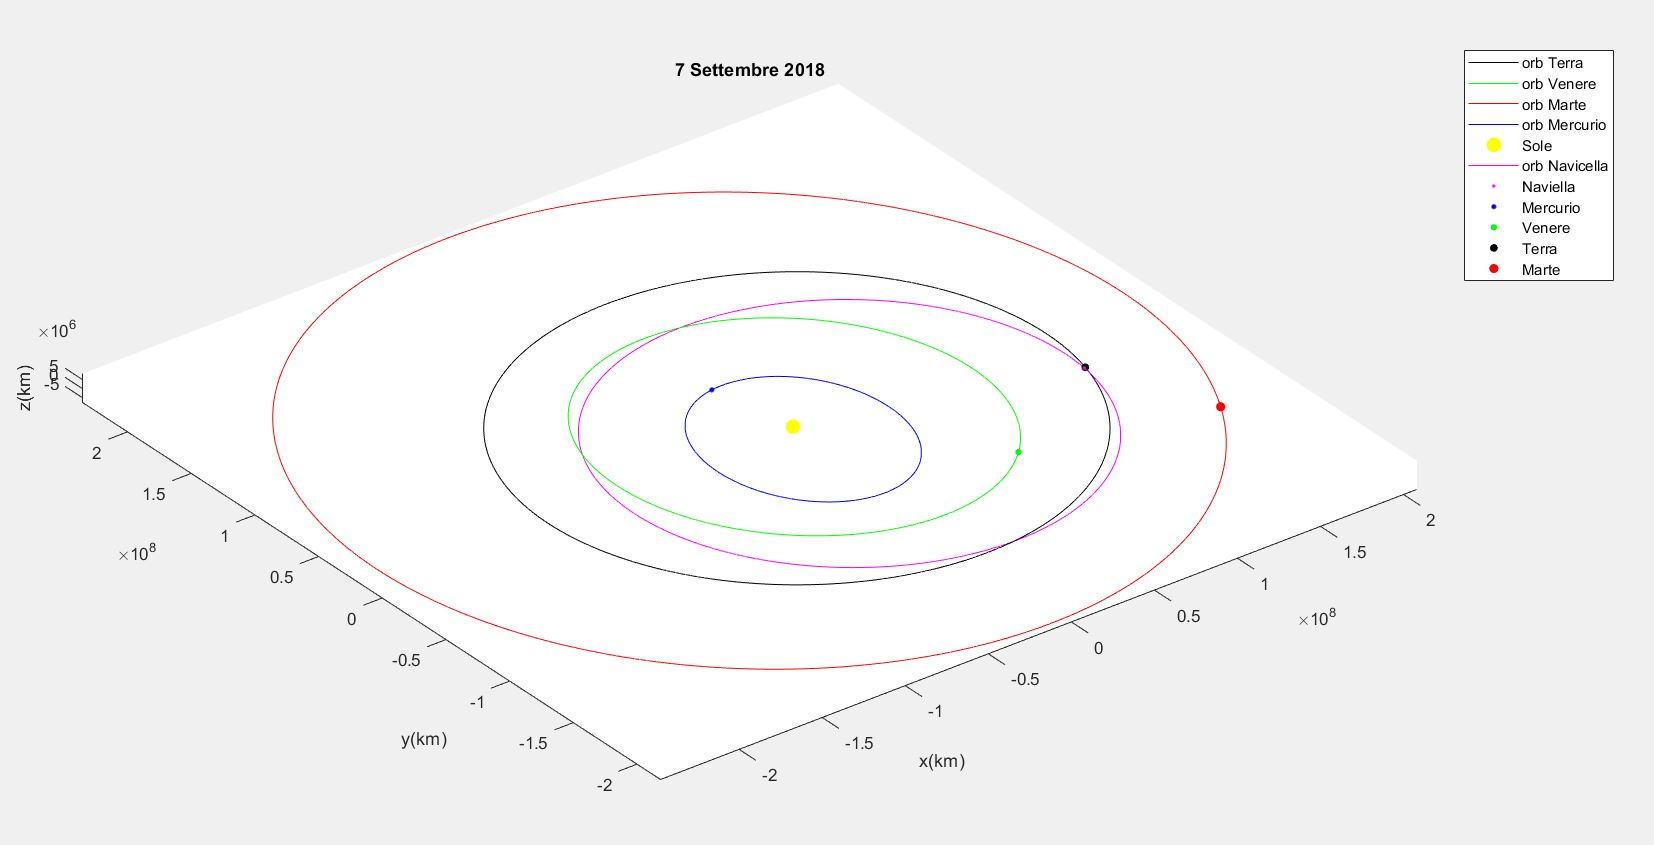
\includegraphics[width=1\textwidth]{Prima_orbita_interplanetaria.png}
\caption{Prima orbita interplanetaria: \newline $a_{orb\_nav} = 1.297e8$ km, $e_{orb\_nav} = 0.215$}
\end{figure}\newline
\begin{figure}[htbp]
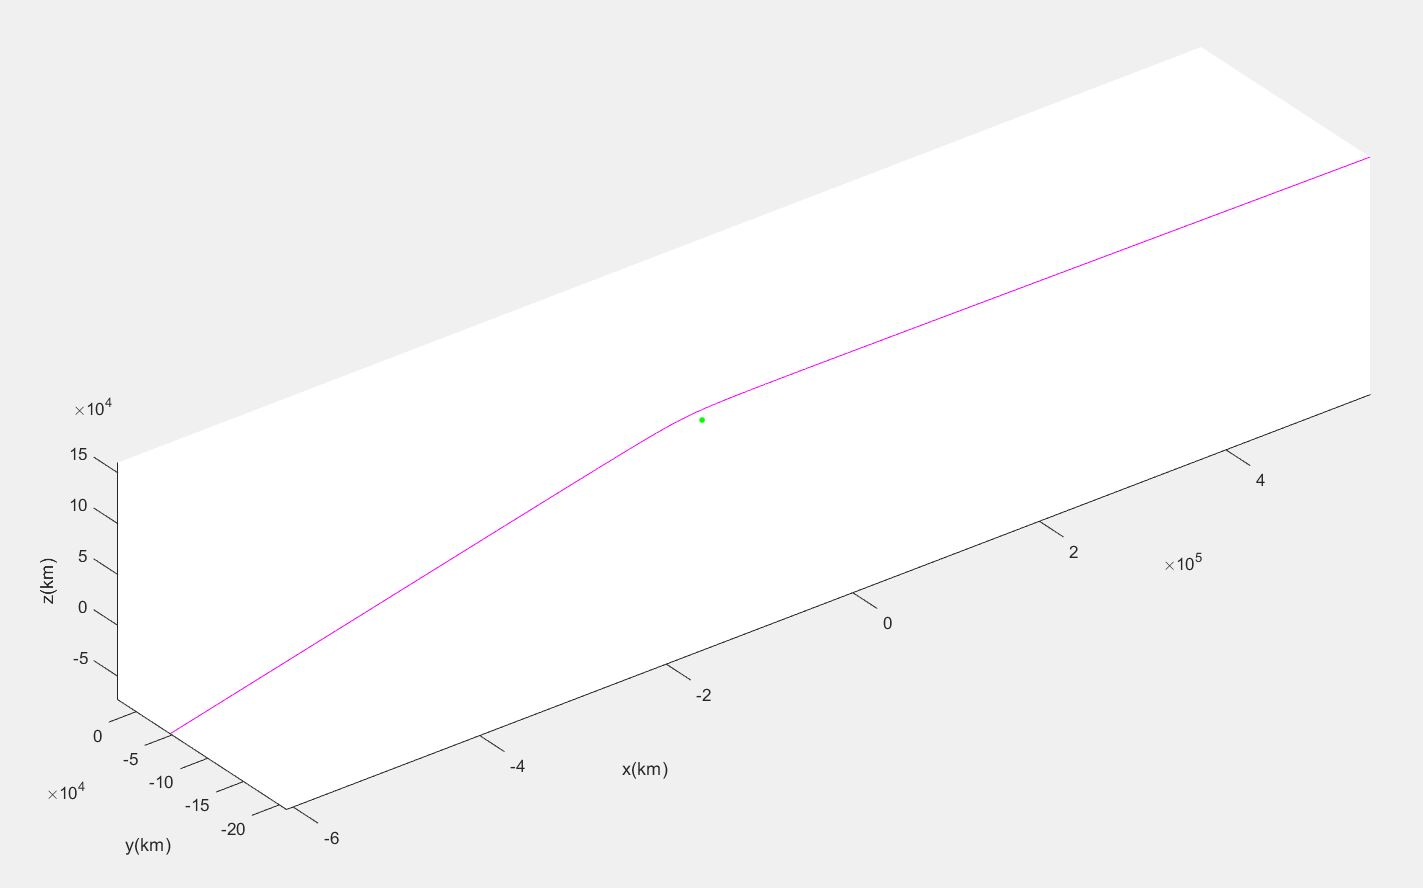
\includegraphics[width=1\textwidth]{fly_by.png}
\caption{Orbita volo ravvicinato su Venere: \newline $r_{p\_hyp} = 25796$ km, $e_{hyp\_orb}$ = 3.574}
\end{figure}\newline
\begin{figure}
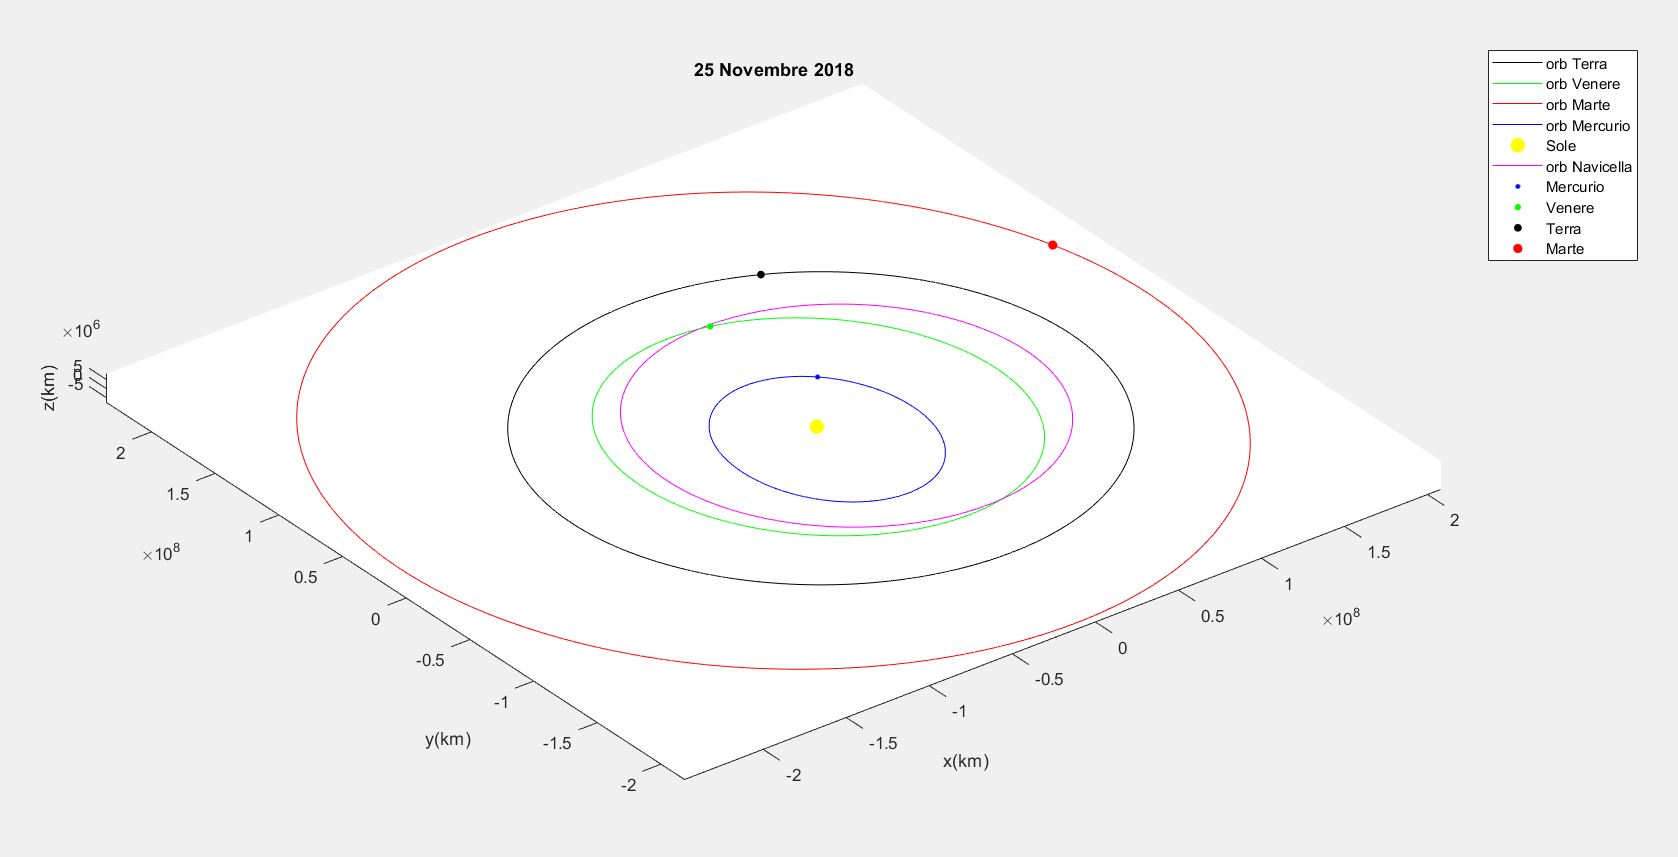
\includegraphics[width=1\textwidth]{Seconda_orbita_interplanetaria.png}
\caption{Seconda orbita interplanetaria: orbita generata successivamente al volo ravvicinato \newline $a_{orb\_nav} = 1.086e8$ km, $e_{orb\_nav} = 0.167$}
\end{figure}\newline
\begin{figure}
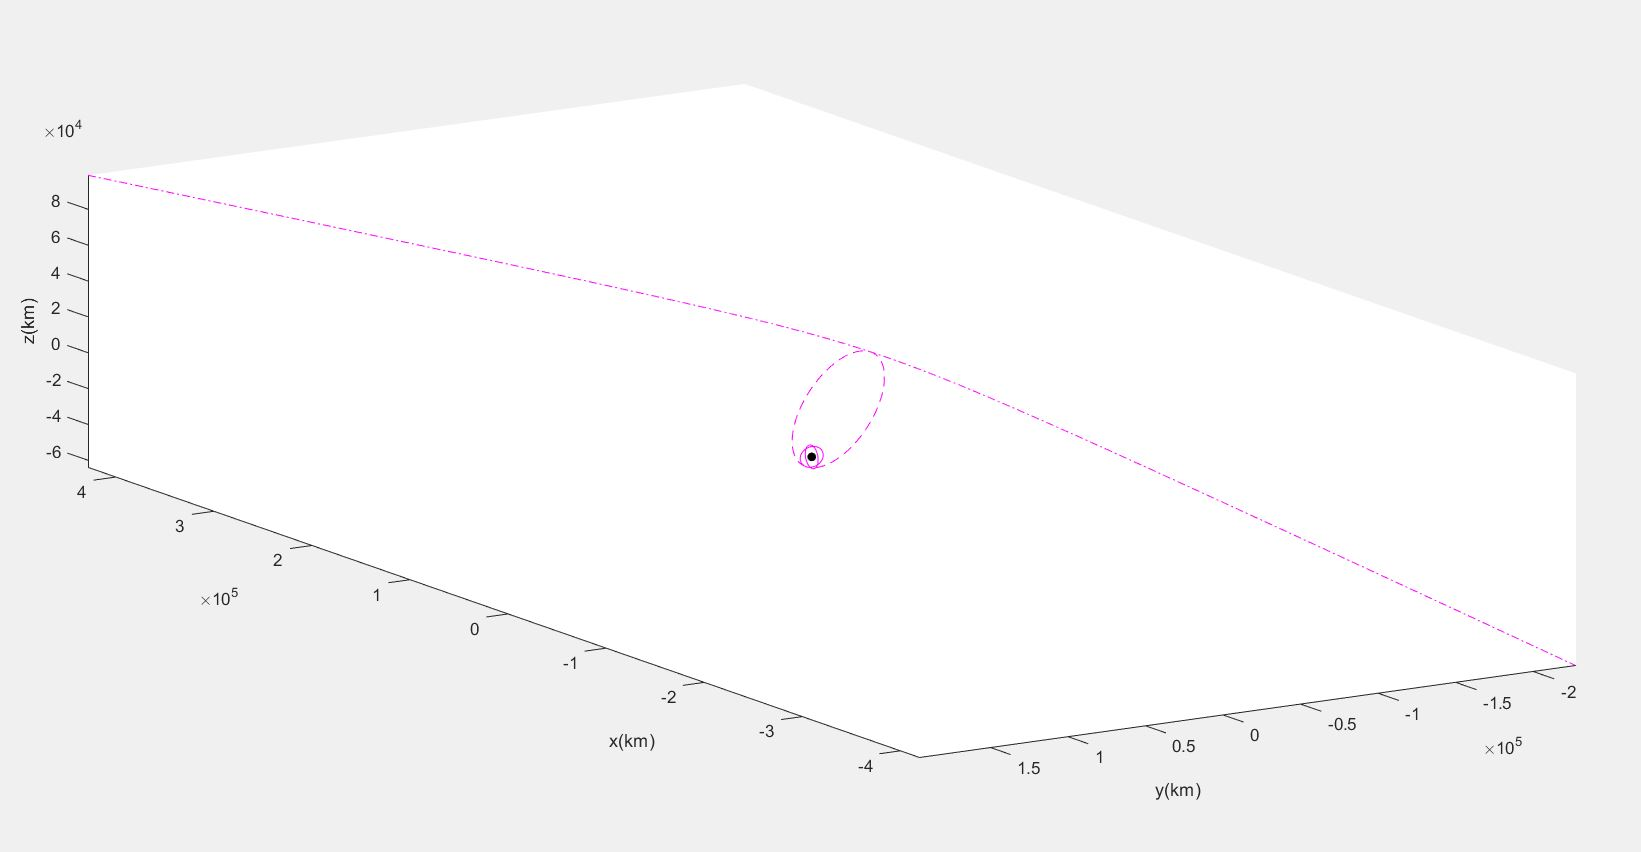
\includegraphics[width=1\textwidth]{Orbite_finali_Venere.png}
\caption{Rappresentazione grafica delle orbite di cattura di Venere: \newline $r_{p\_hyp} = 69757$ km, $e_{hyp} = 9.009$ \newline $a_{ell\_orb} = 38154$ km, $e_{ell\_orb} = 0.828$ \newline $R_{cyrcle\_orb} = 6551$ km, $e_{cyrcle\_orb} = 0$}
\end{figure}\newpage

\subparagraph{Considerazioni finali e problemi\newline}
Prima considerazione è sui punti di Lambert. Per ottenere questi, si son svolte delle simulazioni ''a mano'', andando a settare i valori angolari, fino ad ottenere i risultati cercati. \newline Una seconda considerazione è da farsi sulla simulazione: l'intervallo temporale del calcolo della posizione dei pianeti e della navicella è giornaliera e, a causa di questo, si commettono errori sulla posizione della sonda rispetto alle coordinate nominali. Tutto questo si traduce in una simulazione che nella realtà risulta non del tutto precisa.\newline Una terza limitazione è sull'orbita iperbolica di cattura: come già preannunciato, si desidera che l'iperbole abbia un periasse di circa 6552km. Questa richiesta non si riesce a soddisfare e, come si può notare anche graficamente, siamo costretti ad attuare una manovra in più, che si traduce in uso di carburante.
\subparagraph{Presentazione del codice\newline}
Ottenute tutte le orbite attraverso la funzione \textit{\textbf{gener\_orb.m}}, viene chiamata la funzione \textit{\textbf{simulate\_solar\_system.m}}. Questa come prima cosa si calcola le posizioni dei pianeti nel giorno 1 Gennaio 2018 (J2018) per poi iniziare la vera simulazione, dove nel loop \textit{for} i è l'indice del giorno.\newline Il giorno di partenza della navicella è previsto per il 7 Settembre 2018. Lo script \textit{\textbf{solve\_1\_fly.m}} esegue l'algoritmo di calcolo dei punti che poi verranno passati all'equazione di Lambert, generando l'orbita della prima rotta. Questo script, inoltre, comprende anche la soluzione della rotta dell'uscita dalla sfera d'influenza terrestre (quest'ultima calcolata mediante lo script \textit{\textbf{solve\_exit\_T.m}}). \newline A questo punto la simulazione prosegue finché la norma del vettore distanza tra navicella e Venere sia minore del raggio della SOI del pianeta stesso. \newline Non appena questa condizione risulta verificata, viene lanciato lo script \textit{\textbf{fly\_by.m}} che esegue tutto il calcolo del moto iperbolico, andando anche ad elaborare la nuova orbita interplanetaria causata dalla variazione cinetica della sonda. Questa è calcolata dallo script \textit{\textbf{solve\_2\_fly.m}}. \newline Stessa procedura della prima rotta, si controlla periodicamente che la norma del vettore distanza navicella-Venere sia maggiore del raggio della SOI. Quando ciò risulta non essere più vero, viene chiamata la funzione \textit{\textbf{solve\_sim\_venus.m}}. Questa calcola tutte le orbite fino a quella finale polare.\newline A questo punto, si deve aspettare un tempo pari ad almeno un mese prima di tornare sulla Terra. La missione d'andata può considerarsi conclusa.

\newpage
\part{Seconda parte volo: Venere-Terra}
\paragraph{Introduzione\newline}
Il volo di ritorno consiste in una semplice orbita diretta con trasferimento di Hohmann. Questo mi da un criterio di scelta sull'orbita interplanetaria scelta per la navicella: la richiesta è che si vuole un'ellisse che abbia per afelio il pianeta più interno e per il perielio il pianeta più esterno. Con questa scelta, essendo Venere il pianeta più interno, un piccolo $\Delta(\textit{v})$ mi permette di raggiungere punti più esterni rispetto l'orbita da cui la navicella è partita. Infatti, questo tipo di trasferimento rappresenta un criterio di scelta ottimo in termini di uso di carburante. \newline Quindi in questa sezione viene presentato il problema, le equazioni matematiche, le scelte dovuti a problemi reali 3D ed infine il codice.
\paragraph{Presentazione del problema: trasferimento di Hohmann\newline}
\textit{ }
\begin{figure}[h]
\centering
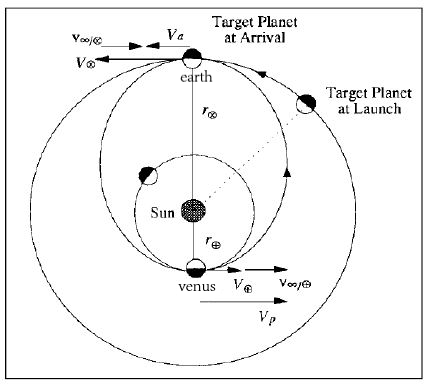
\includegraphics[width=0.75\textwidth]{Hohmann.png}
\caption{Rappresentazione grafica trasferimento di Hohmann da Venere alla Terra, semplificazione 2D}
\end{figure}
\newline
Come già introdotto, il trasferimento di Hohmann prevede che si costruisca un'orbita di rientro dove Venere è il periasse e la Terra l'apoasse. L'ipotesi fatta nell'analisi è che si abbiano orbite 2D, mentre si lascia a considerazioni future l'estensione 3D. \newline Prima cosa, definiamo il semiasse maggiore e le velocità richieste per la navicella spaziale nei punti di incontro con i pianeti (velocità espresse in termini vettoriali):
\[
a_{ellipse} = \frac{r_{earth}+r_{venus}}{2}
\]
\newline
\[
\begin{cases}
\textit{v}_{peri}^{ellipse} = \sqrt{\frac{\mu_{sun}}{a_{ellipse}} \cdot \frac{r_{earth}}{r_{venus}}} \\
\textit{v}_{apo}^{ellipse} = \sqrt{\frac{\mu_{sun}}{a_{ellipse}} \cdot \frac{r_{venus}}{r_{erath}}} \\
\end{cases}
\]
Così noi possiamo calcolare le velocità d'uscita dalla SOI di Venere e d'ingresso nella SOI della Terra:
\[
\begin{cases}
\textit{v}_{\infty}^{venus} = \textit{v}_{peri}^{ellipse} - \textit{v}_{venus} = \textit{v}_{peri}^{ellipse} - \sqrt{\frac{\mu_{sun}}{r_{venus}}} \\
\textit{v}_{\infty}^{earth} =  \textit{v}_{earth} - \textit{v}_{apo}^{ellipse} = \sqrt{\frac{\mu_{sun}}{r_{earth}}} - \textit{v}_{apo}^{ellipse} \\
\end{cases}
\]
A questo punto si calcolano i parametri orbitali prima per l'uscita da Venere:
\[
\textit{a}_{hyp} = -\frac{\mu_{venus}}{(\textit{v}_{\infty}^{venus})^{2}}
\]
\[
\textit{v}_{peri}^{hyp} = \sqrt{\frac{2\mu_{venus}}{R_{cyrcle\_orb}^{venus}}-(\textit{v}_{\infty}^{venus})^{2}}
\]
dove $R_{cyrcle\_orb}^{venus}$ = 6552km è il raggio dell'orbita circolare di parcheggio di Venere; per la Terra:
\[
\textit{a}_{hyp} = -\frac{\mu_{earth}}{(\textit{v}_{\infty}^{earth})^{2}}
\]
\[
\textit{v}_{peri}^{hyp} = \sqrt{\frac{2\mu_{earth}}{R_{cyrcle\_orb}^{earth}}-(\textit{v}_{\infty}^{earth})^{2}}
\]
dove $R_{cyrcle\_orb}^{earth}$ = 6571km e rappresenta il raggio dell'orbita circolare finale.

\subparagraph{Considerazioni 3D e risultati grafici\newline}
Precedentemente si sono enunciate le formule per il calcolo dell'orbita interstellare di ritorno. Si era fatta l'ipotesi di considerare Venere e Terra sullo stesso piano orbitale ma, come sappiamo, nella realtà ciò non è vero. Tuttavia, le equazioni risultano lo stesso valide, a patto di ulteriori vincoli. Prima cosa, consideriamo che l'orbita iperbolica di fuga sia sul piano XY del frame Venere. Con questa ipotesi, il vettore $\textit{v}_{peri}^{ellipse}$, che ricordo essere il vettore velocità della navicella espressa in coordinate Sole, è parallelo alla velocità del pianeta. \newline Seconda ipotesi, sempre riguardante la fuga, per garantire non solo che i vettori velocità risultassero paralleli tra di loro, ma anche che il simulatore non riconosca un nuovo ingresso nella SOI, la navicella deve verificare che il punto spaziale di fuga sia lungo l'asse Y.\newline Con queste ipotesi, il simulatore si calcola le coordinate 3D e velocità della navicella una volta avvenuta la fuga. Quest'ultimi vengono passati nella funzione \textit{\textbf{rv\_to\_orb.m}} che mi restituisce i parametri orbitali, utili per la ricostruzione della traiettoria da seguire. \newline Una terza ipotesi, non trascurabile, è sulla data d'accensione dei motori. Fino ad adesso si è visto solo l'analisi matematica del problema. Ovviamente deve avvenire che la navicella, quando raggiungerà il suo afelio, sia attratto dalla Terra. Per questo, la data è scelta in modo tale che quest'incontro accada ma, in più, sorge un ulteriore problema. Quando la navicella lascia il pianeta, si muove su un'orbita che ha la stessa inclinazione di Venere. Per questo, oltre alla data, bisogna anche programmare un'ulteriore accensione dei motori, per far si che la navicella corregga la sua rotta. \newline Ovviamente, come per la missione d'andata, si settano sia i parametri della posizione d'uscita della SOI, sia quanta variazione cinetica apportare alla navicella nella fase di correzione della traiettoria. \newline
Sono qui riportati i risultati grafici.\newline
\begin{figure}[h]
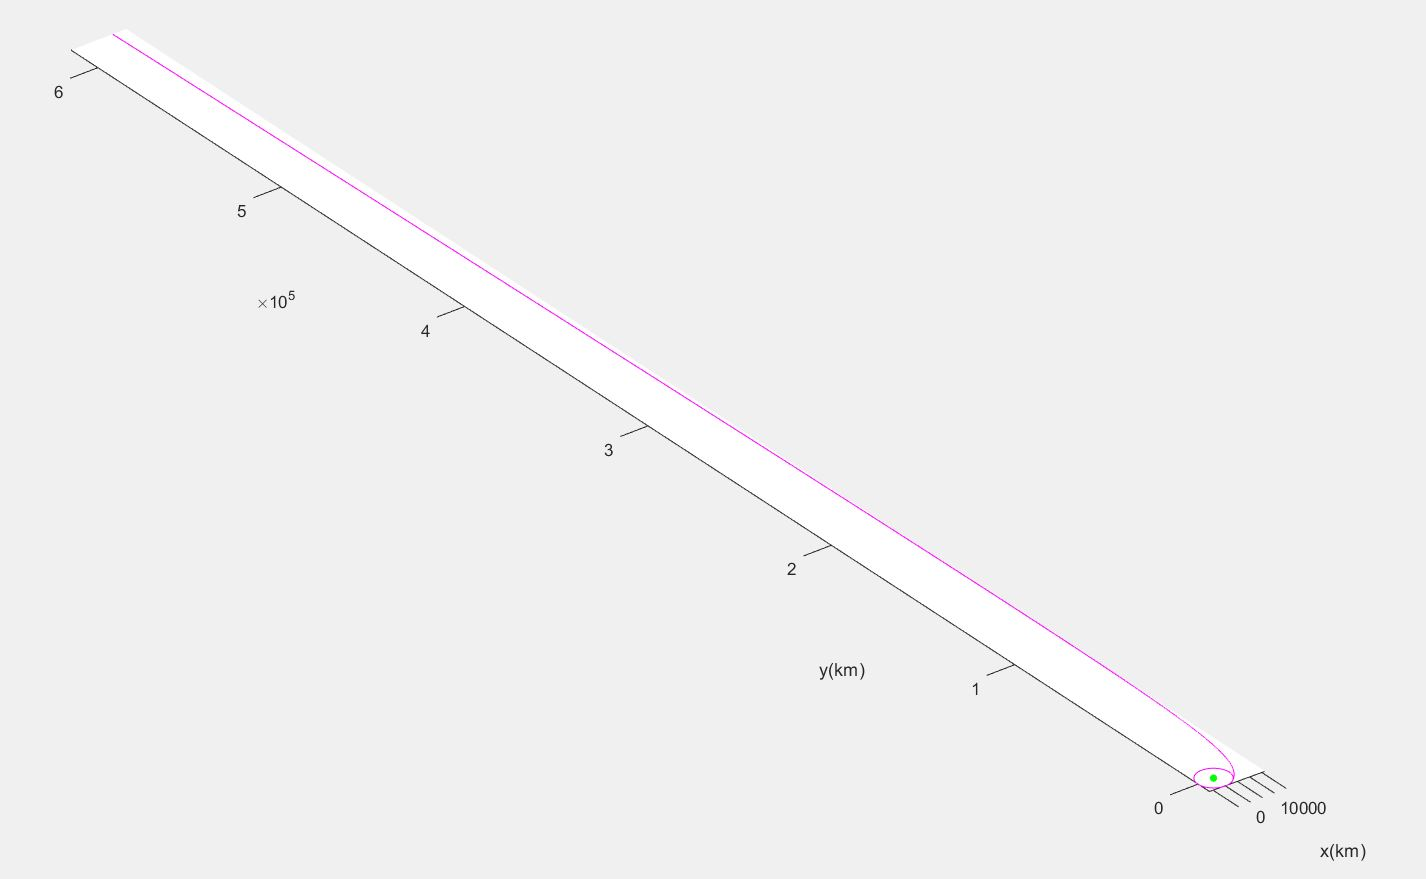
\includegraphics[width=0.75\textwidth]{Exit_venus.png}
\centering
\caption{Orbita iperbolica di fuga da Venere \newline $R_{orb\_cyrcle} = 6552$ km, $e_{orb\_cyrcle} = 0$ \newline $r_{p\_hyp} = 6552$ km, $e_{hyp\_orb} = 1.244$}
\end{figure}
\begin{figure}[h]
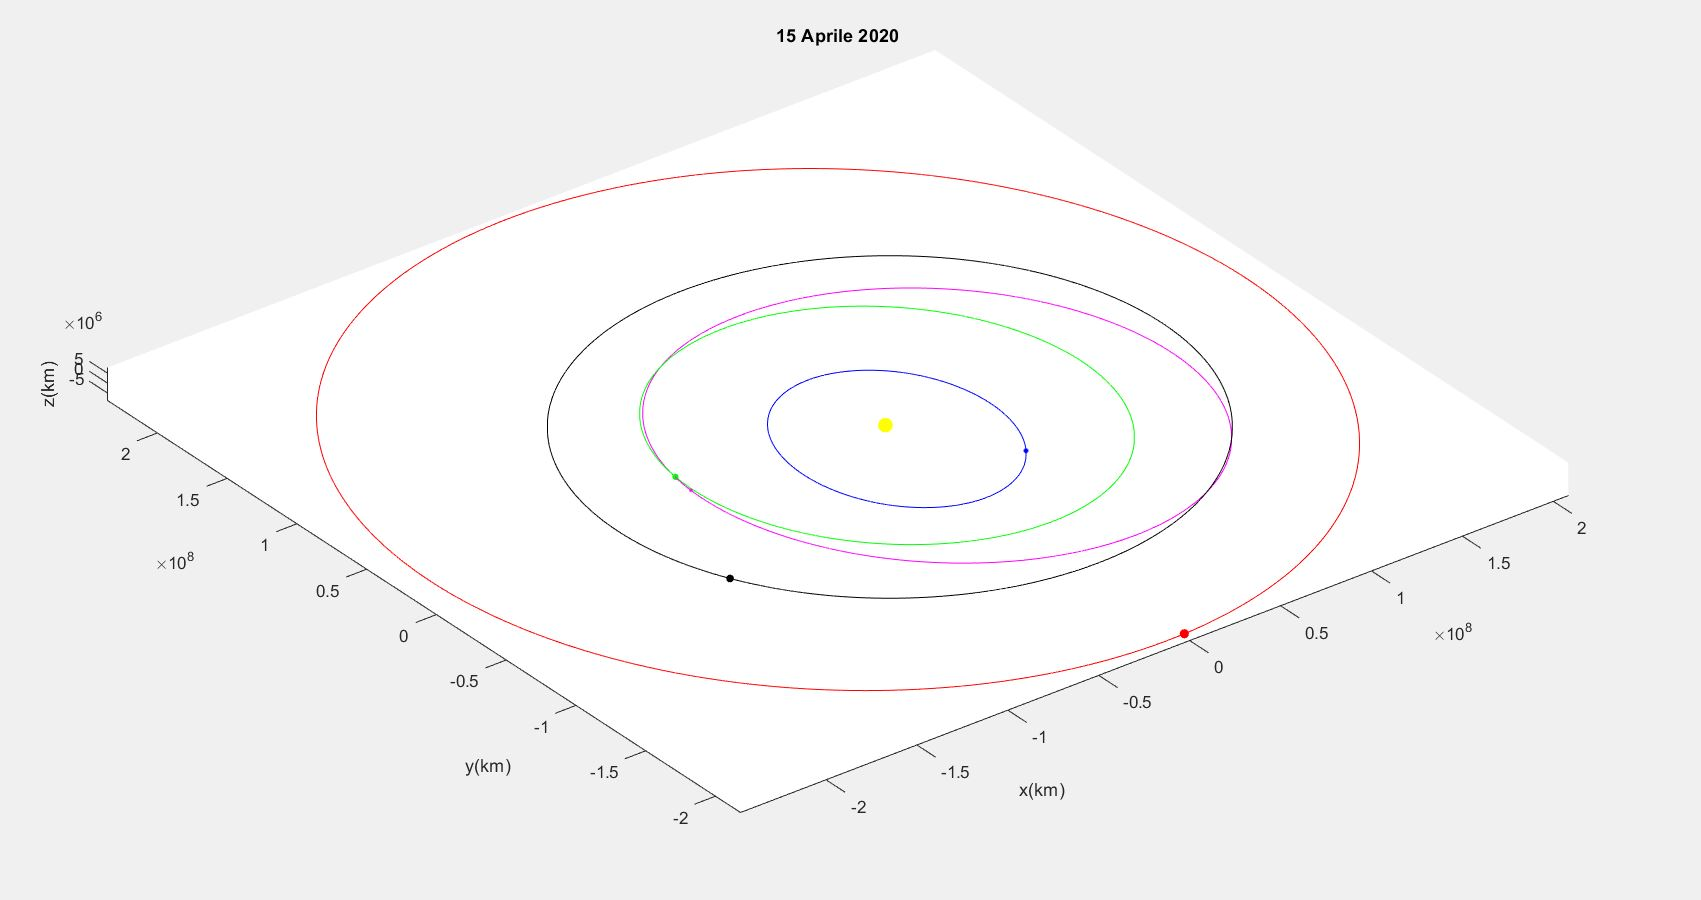
\includegraphics[width=0.75\textwidth]{orbita1.png}
\centering
\caption{Orbita interstellare iniziale di rientro \newline $a_{ell\_orb} = 1.288e8$ km, $e_{ell\_orb} = 0.176$}
\end{figure}
\begin{figure}[h]
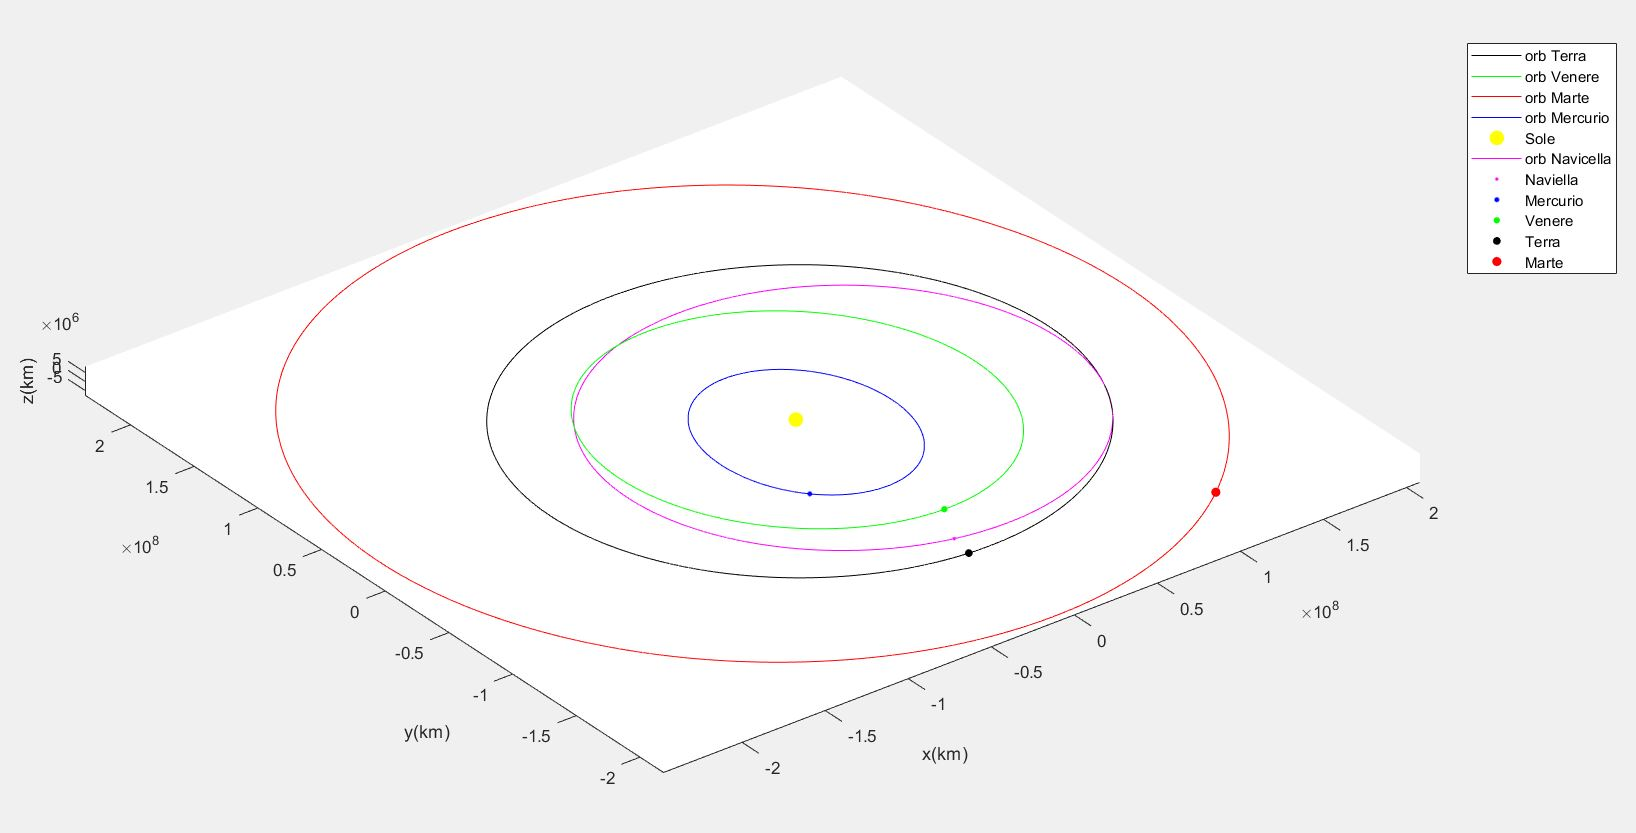
\includegraphics[width=0.75\textwidth]{orbita2.png}
\centering
\caption{Orbita interstellare seguente l'accensione dei motori per la correzione di rotta \newline $a_{ell\_orb} = 1.288e8$ km, $e_{ell\_orb} = 0.176$}
\end{figure}
\begin{figure}[h]
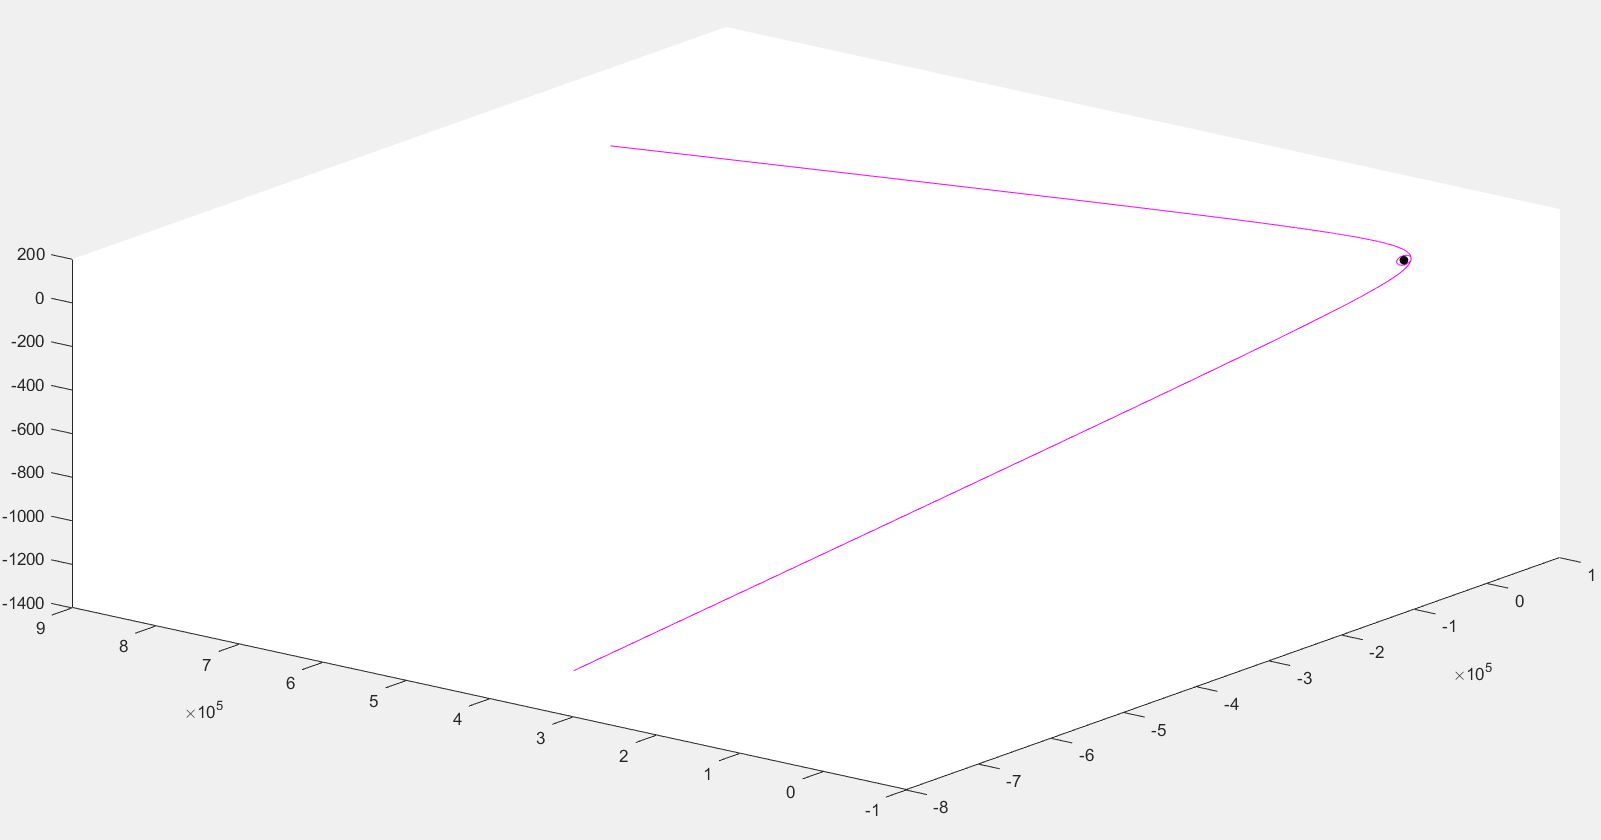
\includegraphics[width=0.75\textwidth]{orbita_finaleT.png}
\centering
\caption{Orbita iperbolica di rientro sulla Terra, con orbita geostazionaria di parcheggio \newline $a_{hyp\_orb} = -69299$ km, $e_{hyp\_orb} = 1.095$ \newline $R_{cyrcle\_orb} = 6569$ km}
\end{figure}
\newpage
\subparagraph{Problemi riscontrati\newline}
Come nella missione d'andata, anche nel ritorno si sono riscontrati dei problemi. \newline Il primo di questi è data dalla simulazione. Come già descritto, il simulatore verifica giorno dopo giorno se la navicella entra nella SOI dei pianeti. Questa sfera, presa come controllo per cambiare il riferimento orbitale della navicella, è una buona approssimazione ma porta nella realtà a dei risultati diversi da quelli simulati. \newline Seconda osservazione è da farsi sull'accensione dei motori: questi si comportano in modo ideale, cioè attivati ci permettono di passare da un'orbita ad un'altra, senza considerare il tempo di combustione necessario per ottenere il risultati desiderati. \newline Una terza osservazione si deve fare sull'orbita ellittica di ritorno: noi abbiamo sì affrontato il problema del rientro attraverso un trasferimento diretto di Hohmann ma, come precedentemente introdotto, l'orbita ottenuta non permette un incontro con la Terra. Per questo si deve effettuare una correzione obbligata nel volo. In più, la simulazione avviene giorno dopo giorno, verificando che la norma del vettore distanza sonda-Terra sia maggiore del raggio della SOI. Quando ciò non è più vera, inizia il calcolo del rientro sulla Terra. Per ottenere i risultati si son settati ''a mano'' sia il giorno di partenza che quanta variazione di velocità apportare nella correzione orbitale. Queste rappresentano un limite del codice che non è in grado di autocalcolarsi i parametri. 
\subparagraph{Presentazione del codice\newline}
Una volta atteso il mese richiesto dalle specifiche di progetto, bisogna aspettare la finestra temporale esatta per il rientro della sonda. \newline Ottenuti i valori di data di partenza e variazione di velocità per affrontare tutto il viaggio (dati salvati nello script \textit{\textbf{day\_burn.m}}), viene chiamato lo script \textit{\textbf{solve\_rientro.m}}. Questo si calcola l'orbita iperbolica d'uscita di Venere e le due ellittiche interstellari. Iniziata la missione di rientro, il simulatore controlla passo dopo passo se la navicella entra nella sfera d'attrazione terrestre. Avvenuto ciò, viene chiamato lo script \textit{\textbf{solve\_SOI\_fin.m}} che calcola l'orbita iperbolica di rientro e quella geostazionaria. Una volta finite le simulazioni di volo, la missione di rientro si definisce conclusa.

\newpage
\part{Framework codice calcolo posizione navicella}
Fino ad adesso si è solo parlato dell'analisi delle orbite, come ottenerle e le proprietà richieste. Il simulatore è in grado di calcolarsi giorno per giorno la posizione dei pianeti e della navicella. Il framework che genera i dati parte dalle stesse equazioni matematiche, andando però a distinguere se l'orbita è circolare, ellittica o iperbolica. \newline Sono qui riportati i passaggi matematici. \newline Per prima cosa, bisogna ricordare la relazione che lega anomalia vera all'anomalia media, passando per la conoscenza dell'anomalia eccentrica: \newline in un'orbita ellittica, di definiscono i tre parametri graficamente come:
\begin{figure}[h]
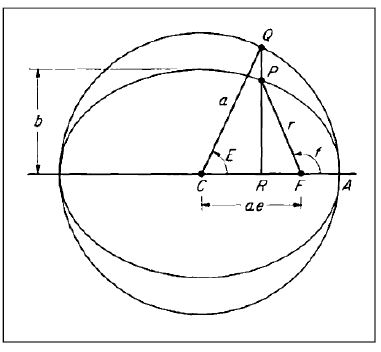
\includegraphics[width=0.75\textwidth]{anomalie.JPG}
\caption{Rappresentazione di: E = anomalia eccentrica; f = anomalia vera (anche chiamata con $\theta$)}
\end{figure}\newline
Qui ci sono le rappresentazioni per un'orbita ellittica, si possono estendere le equazioni sia per il caso di orbita circolare, sia per un'orbita iperbolica. L'anomalia media, valore sempre angolare ma che ha una relazione non lineare con l'anomalia eccentrica, è l'angolo fondamentale per il calcolo della simulazione. Infatti, l'anomalia media, è l'unico valore angolare che ha una relazione lineare nel tempo, per questo verrà calcolato per primo per poi ottenere l'anomalia vera procedendo con le formule inverse. Algoritmicamente, le equazioni per ottenere $\theta(t)$ da M(t) sono scritte nella libreria \textit{\textbf{kepler1.m}} e \textit{\textbf{kepler2.m}}. La differenza tra queste due funzioni è data dal metodo usato per la soluzione numerica. \newline
\subparagraph{Caso orbita ellittica\newline}
Nel caso di un'orbita ellittica, si definiscono:	\newline
M(t) := anomalia media nell'istante temporale t; \newline
E(t) := anomalia eccentrica nell'istante temporale t;\newline
$\theta(t)$ := anomalia vera nell'istante temporale t.\newline
Attraverso delle relazioni trigonometriche, si arriva a trovare le relazioni temporali tra anomalia vera, anomalia eccentrica e media come:
\[
\begin{cases}
tan(\frac{E(t)}{2}) = \sqrt{\frac{1-e}{1+e}}tan(\frac{\theta(t)}{2}) \\
M(t) = E(t) - e \cdot sin(E(t)) \\
M(t) = n\cdot(t-t_{0}) + M(t_{0}) \\
\textit{dove n = $\sqrt{\frac{\mu}{a^{3}}}$} \\
\textit{dove $M(t_{0})$ è il valore di riferimento in un istante di tempo ''iniziale'' $t_{0}$} \\
\end{cases}
\]\newline
Il codice ha come riferimento di ogni pianeta $M(t_{0})$ il valore di anomalia media nel giorno J2018 e, quindi, $t_{0}$ è proprio uguale al tempo trascorso dal giorno 1 Gennaio 2000 al 1 Gennaio 2018. Per questo, possiamo considerare $t_{0}$ dei pianeti nullo, a patto di considerare  $M(t_{0})$ riferito al giorno J2018. Per la navicella l'anomalia media iniziale dipenderà caso per caso dall'orbita in cui la sonda è situata (si pensi a quando ad esempio si ha un cambio di rotta).
\subparagraph{Caso orbita circolare\newline}
Per l'orbita circolare le cose risultano più semplici. Poichè si ha l'uguaglianza M(t) = E(t) = $\theta(t)$ ed \textit{e} = 0, allora le equazioni si semplificano:\newline
\[
\begin{cases}
\theta(t) = n\cdot(t-t_{0}) + \theta(t_{0}) \\
\textit{dove n = $\sqrt{\frac{\mu}{a^{3}}}$} \\
\textit{dove $\theta(t_{0})$ è il valore di riferimento in un istante di tempo ''iniziale'' $t_{0}$} \\
\end{cases}
\]
\subparagraph{Caso orbita iperbolica\newline}
Nel caso dell'orbita iperbolica, le equazioni si complicano ma sono comunque esprimibili in forma chiusa come:
\[
\begin{cases}
cosh(E(t)) = \frac{e+cos(\theta(t))}{1+e\cdot cos(\theta(t))} \\
M(t) = e \cdot sinh(E(t)) - E(t) \\
M(t) = n\cdot(t-t_{0}) + M(t_{0}) \\
\textit{dove n = $\sqrt{\frac{\mu}{a^{3}}}$} \\
\textit{dove $M(t_{0})$ è il valore di riferimento in un istante di tempo ''iniziale'' $t_{0}$} \\
\end{cases}
\]
\newpage

\part{Riferimenti}
- Appunti delle lezioni \newline
- Sito calcolo efemeridi \textit{NASA}: ''\textit{https://ssd.jpl.nasa.gov/horizons.cgi\#top}''\newline
- Sito internet: ''\textit{http://www.bogan.ca/orbits/kepler/orbteqtn.html}''














































\end{document}